\chapter{نتایج و ارزیابی}
\section{مقدمه}
سیستم تشخیص حرکات دست به نقش مهمی در ایجاد تعامل کارآمد بین انسان و ماشین تبدیل شده است. پیاده‌سازی این سیستم با استفاده از تشخیص ژست دست، نوید گستره وسیعی از کاربردها را در صنعت فناوری می‌دهد. در این پروژه، 
معماری‌های گوناگونی مانند شبکه‌های عصبی پیچشی، شبکه‌های حافظه کوتاه‌مدت بلند، و شبکه‌های عصبی چندلایه مورد آزمایش قرار گرفتند تا بهترین پیاده‌سازی برای تشخیص حرکات دست انتخاب شود. 
\\
در این فصل، به بررسی نتایج به‌دست‌آمده از این پروژه پیاده‌سازی شده می‌پردازیم و دقت و عملکرد سیستم در شرایط مختلف را ارزیابی می‌کنیم. همچنین، نقاط قوت و ضعف هر یک از معماری‌های مورد استفاده 
را تحلیل کرده و پیشنهاداتی برای بهبود سیستم ارائه خواهیم داد. هدف این فصل، ارائه یک تحلیل جامع از کارایی سیستم و شناخت دقیق‌تر از عواملی است که می‌توانند به ارتقاء عملکرد آن کمک کنند.


\section{ارزیابی دقت سیستم}
این پروژه با مدل‌های گوناگونی پیاده‌سازی شد تا بتوان بهترین آنها را برای نتیجه نهایی بر روی پهپاد اجرا کرد. نمونه خروجی این مدل‌ها به شرح زیر است.

\begin{table}[h!]
    \centering
    \begin{tabular}{||c c c c||}
     \hline
     \rule{0pt}{3ex} معماری مدل & دوره\LTRfootnote{Epoch} & دقت آموزش & دقت تست  \\ [1.5ex]
     \hline
     \hline
     \rule{0pt}{0.5ex} & & & \\  % Adds space before the first data row, while keeping the vertical lines
     \lr{MLP} & 6 & 7 & 1 \\ [2.5ex]
     \lr{CNN} & 7 & 8 & 2 \\ [2.5ex]
     \lr{LSTM} & 5 & 8 & 3 \\ [2.5ex]
     \hline
    \end{tabular}
    \caption{جدول ارزیابی  دقت مدل‌ها}
    \label{table:2}
\end{table}

\section{دقت تشخیص برای ۹ ژست‌ دست}
% تحلیل دقت مدل‌ها در شرایط مختلف
% مقایسه دقت بین معماری‌های مختلف (CNN، LSTM، MLP)
% در این بخش، نتایج ارزیابی مدل برای تشخیص ۹ ژست مختلف دست ارائه شده است. معیارهای ارزیابی شامل دقت، یادآوری، نمره \lr{F1} و حمایت (تعداد نمونه‌ها)
% برای هر یک از ژست‌ها می‌باشد. این معیارها به تفصیل در جدول زیر نمایش داده شده‌اند تا عملکرد مدل در طبقه‌بندی ژست‌ها مشخص گردد.

در این بخش، نتایج ارزیابی مدل برای تشخیص ۹ ژست مختلف دست ارائه شده است. معیارهای ارزیابی شامل معیار صحت \LTRfootnote{Precision}، فراخوانی\LTRfootnote{Recall}، معیار \lr{F1} و
تعداد نمونه‌ها برای هر یک از ژست‌ها می‌باشد.


\subsection{دقت}
دقت مدل معیاری است که نشان می‌دهد یک مدل یادگیری ماشینی چقدر قادر به پیش‌بینی یا تصمیم‌گیری بر اساس داده‌ها است. این معیار به صورت مجموع مثبت و منفی واقعی تقسیم بر تعداد کل نمونه ها محاسبه می شود.
\\
دقت بصری ترین معیار عملکرد است و برابر نسبت مشاهدات پیش بینی شده درست به کل مشاهدات است. این معیار می‌تواند برای مقایسه عملکرد مدل‌های مختلف یا ارزیابی اثربخشی یک مدل خاص برای یک کار معین استفاده شود.
\\
دقت به صورت مجموع مثبت و منفی واقعی تقسیم بر تعداد کل نمونه ها محاسبه می شود. همچنین این معیار زمانی مناسب است که کلاس ها به خوبی متعادل باشند و هزینه های مثبت کاذب و منفی کاذب مشابه باشد.
\[ Accuracy = \frac{True \, Positive + True \, Negative}{True \, Positive + True \, Negative +  False \, Positive + False \, Negative} \]

\subsection{صحت}
صحت یک معیار آماری برای ارزیابی کیفیت یک مدل پیش‌بینی است. این یکی از معیارهای کلیدی است که برای تعیین عملکرد یک مدل، به ویژه در وظایف طبقه بندی استفاده می شود. صحت نسبت مثبت واقعی به مجموع مثبت های واقعی و مثبت کاذب (نمونه هایی که به اشتباه به عنوان مثبت شناسایی شده اند) است.
\\
صحت بالا نشان دهنده این است که یک مدل در جلوگیری از مثبت کاذب خوب عمل می‌کند، به عنوان مثال، نمونه های منفی را به عنوان مثبت طبقه بندی نمی کند. این امر به ویژه در برنامه هایی که هزینه مثبت کاذب بالا است، اهمیت دارد. 

\[ Precision = \frac{True \, Positive}{True \, Positive - False \, Positive} \]

\subsection{فراخوانی}
معیار فراخوانی که به عنوان نرخ مثبت واقعی نیز شناخته می‌شود، این معیار برابر نمونه‌های داده‌ای است که یک مدل یادگیری ماشینی به درستی آن‌ها را تشخیص داده نسبت به کل نمونه‌های آن کلاس است.
\\
فراخوانی زمانی استفاده می‌شود که به حداقل رساندن منفی های کاذب از اهمیت ویژه ای برخوردار باشد. بدین صورت که هزینه بر روی مثبت کاذب کم باشد و یا هزینه از دست دادن مثبت واقعی زیاد باشد. 
\[ Recall = \frac{True \, Positive}{True \, Positive - False \, Negative} \]

\subsection{امتیاز \lr{F1}}
امتیاز \lr{F1} معیاری برای میانگین هارمونیک دقت و یادآوری است. امتیاز \lr{F1} که معمولاً به عنوان معیار ارزیابی در طبقه‌بندی باینری و چند کلاسه استفاده می‌شود، صحت و یادآوری را در یک متریک واحد ادغام می‌کند تا درک بهتری از عملکرد مدل به دست آورد.
\\
امتیاز \lr{F1} یک معیار مفید برای اندازه‌گیری عملکرد مدل‌های طبقه‌بندی برای زمانی است که داده‌ها نامتعادل‌اند، زیرا نوع خطاها - مثبت کاذب و منفی کاذب - و نه فقط تعداد پیش‌بینی‌های نادرست را در نظر می‌گیرد.


\[ F1  = \frac{2 \times Precision \times Recall}{Precision + Recall} \]


\begin{figure}[h]
    \centering
    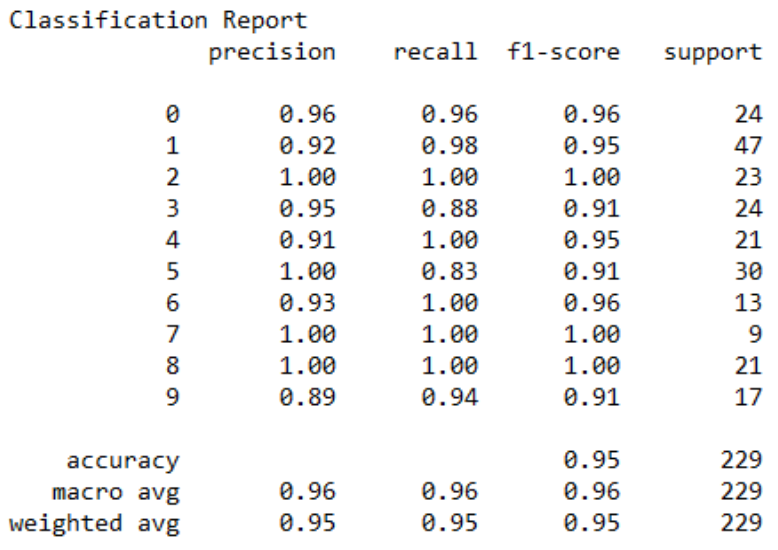
\includegraphics[width=0.7\textwidth]{textchart.png}
    \caption{جدول عملکرد طبقه بندی دقت تشخیص ژست دست برای مدل \lr{MLP}}
\end{figure}


اعداد نشان داده‌شده به خوبی نمایانگر عملکرد مدل هستند. 


\section{نمودار‌های دقت و خطا بر حسب دوره}
% بررسی و تحلیل نرخ خطاها
دلایل خطا و راهکارهای پیشنهادی برای کاهش آنها






\begin{figure}[h]
    \centering
    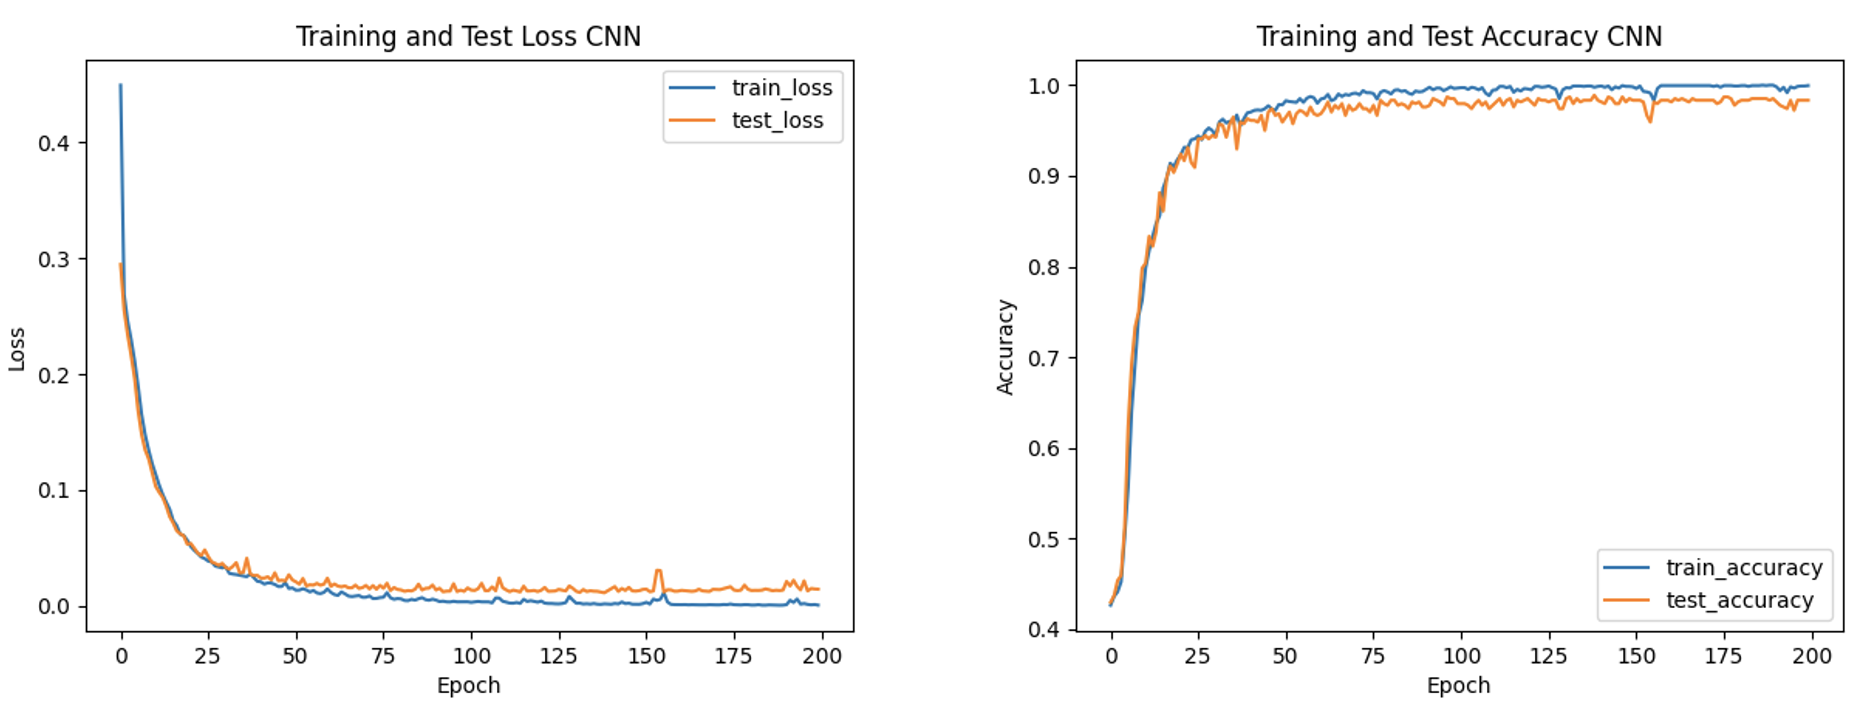
\includegraphics[width=1\textwidth]{CNN.png}
    \caption{نمودار روند دقت و خطا بر حسب دوره در داده‌های آموزش و تست در مدل \lr{CNN}}
\end{figure}




\section{عملکرد زمان‌بندی}


\section{سرعت اجرای برنامه}
زمان پاسخگویی سیستم
تاثیر استفاده از کارت گرافیکی بر سرعت

\section{سخت‌افزار مورد نیاز}
این پروژه باید به گونه‌ای اجرا می‌شد که بر روی ساده‌ترین سیستم‌های کامپیوتری نیز قابل اجرا باشد، زیرا سخت‌افزار پهپادها به‌طور معمول دارای پردازنده‌های ضعیف‌تری هستند. همچنین، استفاده از کارت گرافیکی ممکن نبود، چرا که 
پهپادها فاقد کارت گرافیکی می‌باشند. معماری‌های پیاده‌سازی شده به نحوی طراحی شدند که تعادل میان دقت و بهره‌وری از سخت‌افزار حفظ شود، به طوری که هم قابلیت اجرای زمان واقعی داشته باشند و هم امکان پیاده‌سازی آن‌ها بر روی پهپاد 
فراهم باشد. از این رو، معماری‌ها به گونه‌ای پیاده‌سازی شدند که بر روی پردازنده اجرا شوند و میزان استفاده از پردازنده برای آن‌ها به شرح زیر است:


\begin{table}[h!]
    \centering
    \begin{tabular}{||c c c||}
     \hline
     \rule{0pt}{3ex}معماری مدل & پردازنده & فضای ذخیره‌شده \\ [1.5ex]
     \hline
     \hline
     \rule{0pt}{0.5ex} & & \\  % Adds space before the first data row, while keeping the vertical lines
     \lr{MLP} & 6 & 7 \\ [2.5ex]
     \lr{CNN} & 7 & 8 \\ [2.5ex]
     \lr{LSTM} & 5 & 8 \\ [2.5ex]
     \hline
    \end{tabular}
    \caption{جدول ارزیابی سخت‌افزار موردنیاز مدل‌ها}
    \label{table:1}
\end{table}







\section{جمع‌بندی}
